\begin{figure}[!t]
\centering
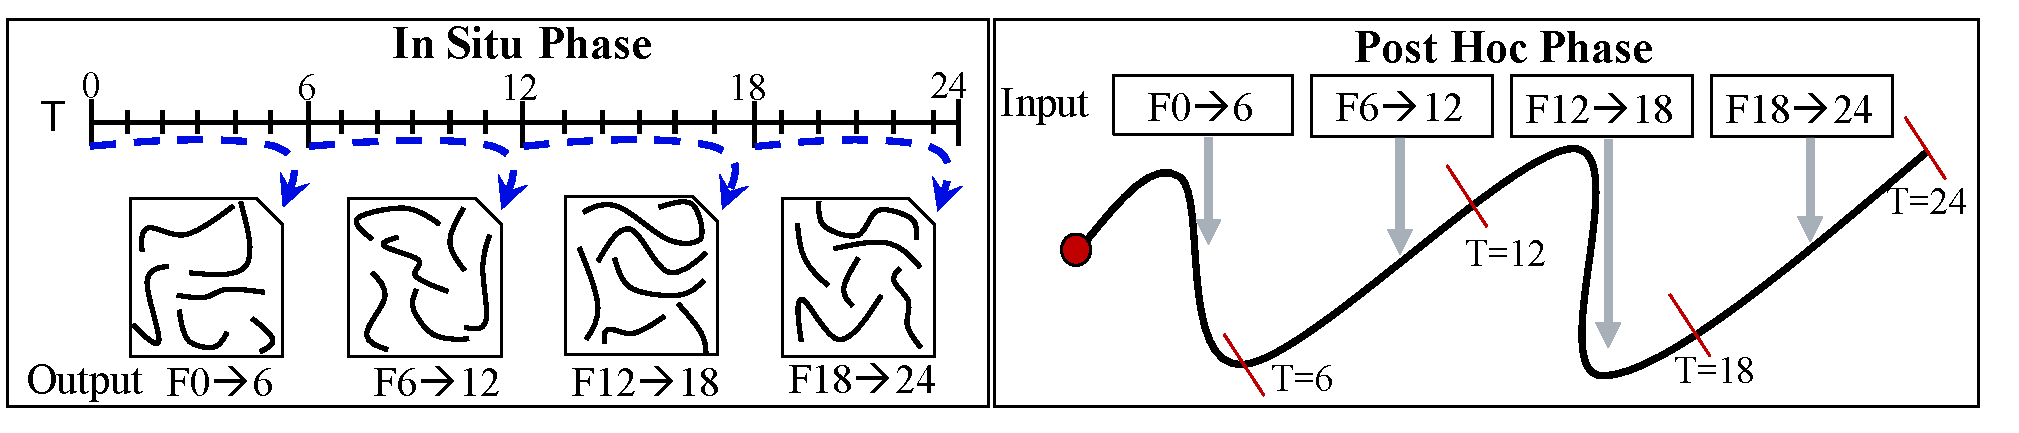
\includegraphics[width=\linewidth]{Images/Phases2.pdf}
\caption{\fix{The two phases of Lagrangian analysis: in situ and post hoc. The in situ phases involves computing flow maps over temporally non-overlapping intervals. During post hoc analysis, the flow maps can be interpolated to explore the flow behavior.} \fix{Does this figure need to change?}}
\vspace{-6mm}
\label{fig:phases}
\end{figure}
